\subsection{Solução}

Para solucionar o problema da falta de comunicação entre diferentes BPMs com atividades compartilhadas, foi idealizada uma funcionalidade para integrar múltiplos BPMs com atividades que se repetem com a criação de um grande BPM agregado com múltiplas atividades iniciais.

Cada atividade inicial representa o início de um BPM, podendo existir uma ou mais atividades iniciais (como na figura~\ref{fig:bpl_completo}).
Como cada atividade inicial ainda representa uma instância daquele BPM, as informações de atividades compartilhadas entre BPMs são compartilhadas entre instâncias destes BPMs.

\begin{sidewaysfigure}
    \centering
    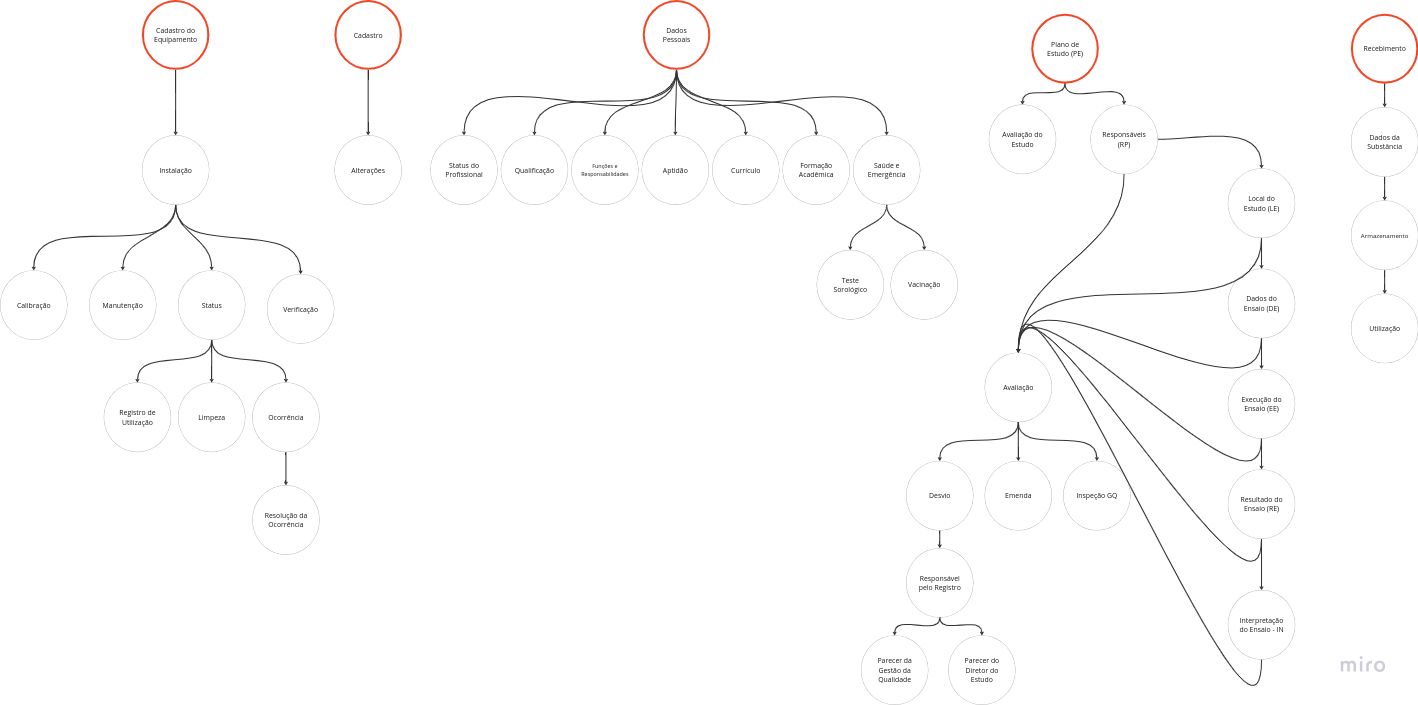
\includegraphics[width=1\textwidth]{imgs/BPL/bpl_completo.png}
    \caption{Estrutura de workflows BPL todos em um mesmo diagrama. Neste caso, cada atividade inicial (em vermelho) pode ser iniciada como uma instância no Flux.}
    \label{fig:bpl_completo}
\end{sidewaysfigure}

Um usuário (Ou múltiplos) criam instâncias dos BPMs compartilhados e, ao executar uma atividade compartilhada, podem escolher com quais instâncias irá compartilhar as informações contidas no mesmo.
Como exemplo, se tivermos a execução de uma atividade de pedido de exame, e existam instâncias de laboratórios de análise de amostras que compartilham da mesma atividade, o médico (usuário executando a atividade de pedido de exame) pode escolher para qual instância de laboratório essa atividade será compartilhada (como na figura~\ref{fig:arvore_medico_tecnico} citada anteriormente).

O administrador que gerencia o workflow também pode configurar permissões de atividades filhas da atividade compartilhada, podendo mostrar um fluxo de trabalho apenas para o laboratório de análise de amostras, ou seja, atividades sobre como será feito a análise estarão disponíveis apenas para os laboratórios, dando maiores possibilidades para o compartilhamento de atividades únicas.

Isso se torna útil quando se deve fazer um pedido de exame para um laboratório, o laboratório deve realizar a análise e disponibilizar os resultados para quem requisitou do exame. Neste caso, ocorre uma troca de informações assíncrona: um usuário executa uma atividade que fica disponibilizada para execução por outro usuário. Este a executa e disponibiliza o resultado para o primeiro usuário, que continua com seu fluxo de trabalho após obter os resultados.

Esta troca de informações possibilita uma maior intercomunicação entre setores da organização e aumenta a integração do LIMS onde ele está instalado, pois todas as informações, tanto de horário de requisição, quanto recebimento pelo outro usuário e execução do fluxo de trabalho compartilhado ficam armazenados no mesmo workflow.

\subsubsection{Mudanças no Flux para sua implementação}

Enquanto a BPMN permite múltiplas maneiras de iniciar um processo, ela permite apenas uma atividade inicial em um diagrama de processo, representado por um único evento de início.

Como uma organização pode ter múltiplas equipes trabalhando em focos diferentes, é necessário a divisão em diversos workflows para que todos os processos estejam modelados para que fluxos de trabalho possam ser diagramados e executados.

Como um mesmo workflow pode ter troca de informações com alguma parte de outros workflows, foi idealizado uma nova funcionalidade para um workflow no Flux: Múltiplas atividades iniciais que compartilham atividades entre instâncias no meio de sua execução.

Cada possível atividade inicial do workflow pode ser utilizada para criar uma instância diferente do workflow, já que cada uma dessas atividades representa um tipo de execução diferente do workflow (na figura~\ref{fig:segunda_implementacao}, uma atividade inicial é para cadastro de pacientes e a outra para cadastro de técnicos de laboratório).

Com um workflow com múltiplas atividades iniciais, é possível ter atividades que, ao serem executadas, serão disponibilizadas para outros usuários que utilizam este workflow, independente da instância que estiverem executando. Assim, usuários que estão executando atividades em uma parte do workflow (partindo de uma atividade inicial) compartilham informações com outros usuários (partindo de outra atividade inicial).

Com a execução de dois workflows agregados, cada execução iniciando de uma atividade inicial diferente, é possível o compartilhamento das atividades que contém um processo idêntico entre os dois workflows agregados, disponibilizando as informações para as instâncias selecionadas.

Desta forma, aumenta-se a integração do sistema por haver a troca de informações entre processos de trabalho diferentes dentro de uma mesma organização, disponibilizando a cooperação entre usuários do mesmo sistema.